%% LyX 2.3.6.1 created this file.  For more info, see http://www.lyx.org/.
%% Do not edit unless you really know what you are doing.
\documentclass[english,xcolor=svgnames, handout]{beamer}
\usepackage{amstext}
\usepackage{fontspec}
\setcounter{secnumdepth}{3}
\setcounter{tocdepth}{3}
\usepackage{calc}
\usepackage{graphicx}
\ifx\hypersetup\undefined
  \AtBeginDocument{%
    \hypersetup{unicode=true}
  }
\else
  \hypersetup{unicode=true}
\fi

\makeatletter
%%%%%%%%%%%%%%%%%%%%%%%%%%%%%% Textclass specific LaTeX commands.
% this default might be overridden by plain title style
\newcommand\makebeamertitle{\frame{\maketitle}}%
% (ERT) argument for the TOC
\AtBeginDocument{%
  \let\origtableofcontents=\tableofcontents
  \def\tableofcontents{\@ifnextchar[{\origtableofcontents}{\gobbletableofcontents}}
  \def\gobbletableofcontents#1{\origtableofcontents}
}

%%%%%%%%%%%%%%%%%%%%%%%%%%%%%% User specified LaTeX commands.

% you can play with different themes and color themes to find your favorite combination.
\mode<presentation> {
  \usetheme{Luebeck}
  \usecolortheme{beaver}
  \beamertemplatenavigationsymbolsempty
}

\usepackage{mathtools}
\usepackage{graphicx} % for including images
\usepackage{pgf} % for logo
\usepackage{colortbl}
\usepackage{booktabs}
\usepackage{emoji}
\usepackage{listings}
\usepackage[many]{tcolorbox}
\usepackage{tabularx}
\usepackage{array}
\tcbuselibrary{skins}
%\usepackage{fdsymbol} % for card symbols


\newcolumntype{Y}{>{\raggedleft\arraybackslash}X}
\tcbset{tab2/.style={enhanced, fontupper=\small,
colback=lightgray!10!white,colframe=cobalt!50!black,colbacktitle=lightsteelblue!40!white,
coltitle=black,center title}}

\newcommand\boldblue[1]{\textcolor{cobalt}{\textbf{#1}}}
\newcommand\boldorange[1]{\textcolor{burntoranger}{\textbf{#1}}}
\def\*#1{\mathbf{#1}}

\date{} % Date, can be changed to a custom date


\definecolor{blue}{RGB}{38, 122, 181}
\definecolor{orange}{RGB}{255, 128, 0}
\definecolor{lorange}{RGB}{255, 178, 102}
\definecolor{llorange}{RGB}{255, 229,204 }
\definecolor{verylightgray}{RGB}{246, 246, 246}
\definecolor{cobalt}{HTML}{0047AB}
\definecolor{lightsteelblue}{HTML}{b0c4de}


\setbeamertemplate{itemize item}{\color{orange}$\blacksquare$}
\setbeamertemplate{itemize subitem}{\color{orange}$\blacktriangleright$}

\usepackage{tcolorbox}

\newcommand\blfootnote[1]{%
  \begingroup
  \renewcommand\thefootnote{}\footnote{#1}%
  \addtocounter{footnote}{-1}%
  \endgroup
}

\makeatother

\usepackage{polyglossia}
\setdefaultlanguage[variant=american]{english}
\begin{document}
\title[\textcolor{gray}{ST1101\hspace{4.45cm}\insertframenumber/\inserttotalframenumber}]{\textcolor{orange}{Statistik och Dataanalys I}}
\subtitle{\textcolor{orange}{Föreläsning 19 - Inferens i linjär regression -
populationsmodell och samplingfördelning}}
\author[\textbf{\textcolor{gray}{Statistik och Dataanalys I}}]{\textbf{Oskar Gustafsson}\\
\vspace{0.2cm}
\vspace{-0.3cm}
}
\institute[Stockholms universitet]{Statistiska institutionen\\
Stockholms universitet}

\makebeamertitle

\begin{frame}{\textbf{\textcolor{orange}{Översikt}}}
\begin{itemize}
\item \textbf{\textcolor{blue}{Inferens i enkel linjär regression\bigskip{}
}}
\item \textbf{\textcolor{blue}{Regression som sannolikhetsmodell\bigskip{}
}}
\item \textbf{\textcolor{blue}{Samplingfördelning regression\bigskip{}
}}
\end{itemize}
\end{frame}

\begin{frame}{\textbf{\textcolor{orange}{Samband - hälsovårdsbudget och livslängd}}\hspace{0.5cm}
\includegraphics[scale=0.6]{figs/lifespan_data_badge}}
 
\begin{center}
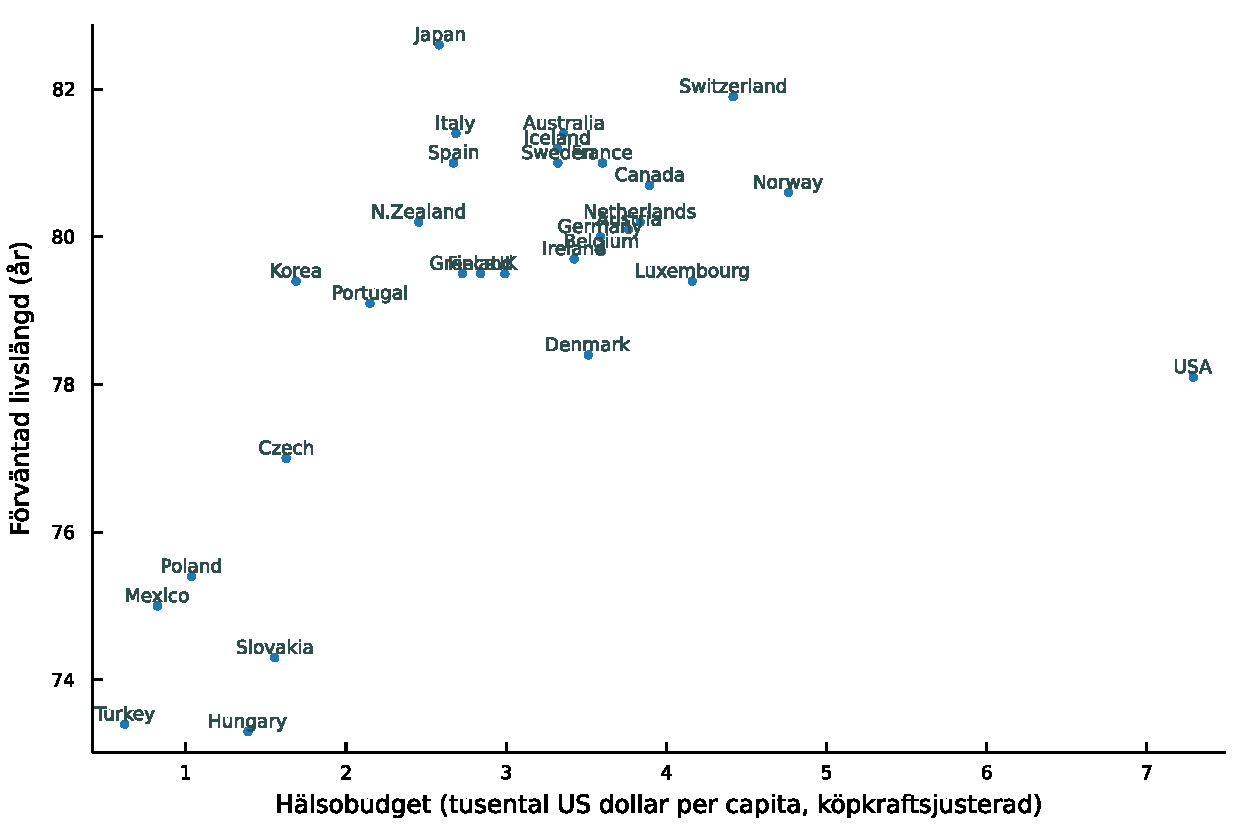
\includegraphics[scale=0.4]{figs/healthdata_text}
\par\end{center}

\blfootnote{Källa: boken \href{https://users.aalto.fi/~ave/ROS.pdf}{\underline{\textcolor{blue}{'Regression and other stories'}}} och OECD.}
\end{frame}

\begin{frame}{\textbf{\textcolor{orange}{Regression - hälsovårdsbudget och livslängd}}}
\begin{center}
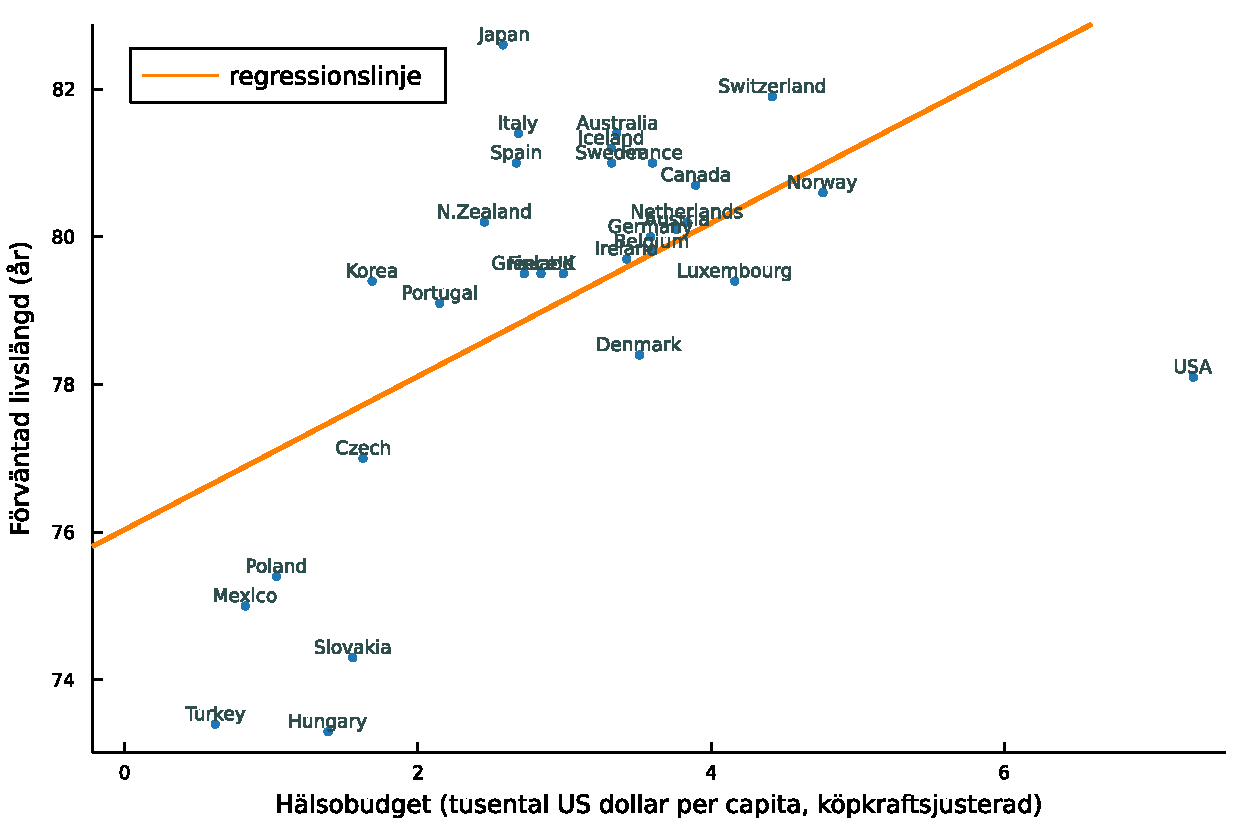
\includegraphics[scale=0.4]{figs/healthdata_text_fit}
\par\end{center}

\end{frame}

\begin{frame}{\textbf{\textcolor{orange}{Anpassad regressionslinje och tolkning}}}
\begin{itemize}
\item Skattad regressionslinje hälsobudget ($x$) $\rightarrow$ livslängd
($y$)
\begin{align*}
\text{lifespan} & =76.035+1.03757\cdot\mathrm{\text{spending}}\\
\\
\hat{y} & =\underset{b_{0}}{\underbrace{76.035}}+\underset{b_{1}}{\underbrace{1.038}}\cdot x
\end{align*}
\smallskip{}
\item Tolkning \textbf{\textcolor{blue}{intercept $b_{0}$}}: \textbf{\textcolor{orange}{genomsnittlig}}
livslängd är ca $76$ år om $\text{spending}=0$.\bigskip{}
\item Tolkning \textbf{\textcolor{blue}{lutning $b_{1}$}}: \textbf{\textcolor{orange}{genomsnittlig}}
livslängd ökar med $1.038$ år om \texttt{spending} ökar med 1 (tusen
US dollar per capita).
\end{itemize}
\end{frame}

\begin{frame}{\textbf{\textcolor{orange}{Inflytelserika observationer}}}
\begin{center}
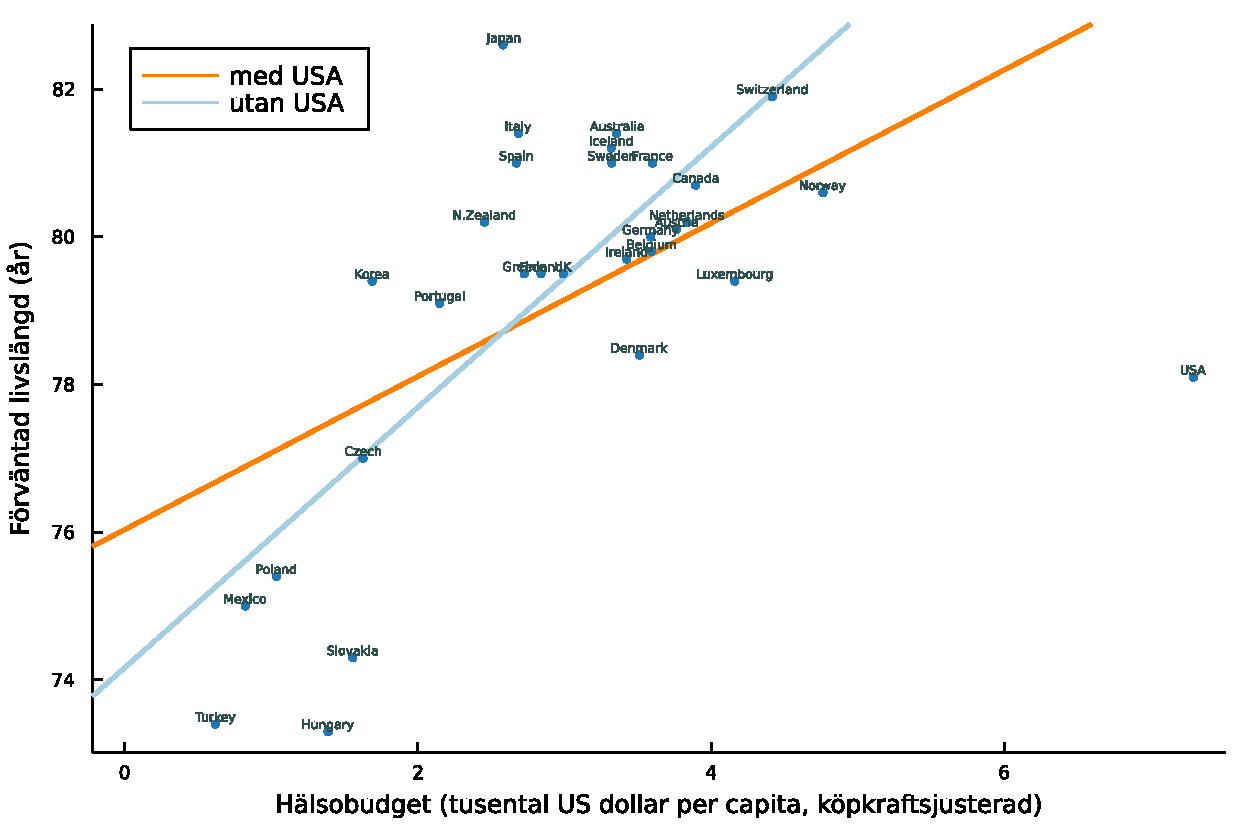
\includegraphics[scale=0.36]{figs/healthdata_text_fit_USA}
\par\end{center}
\begin{itemize}
\item Med USA
\[
\text{lifespan}=76.035+1.038\cdot\mathrm{\text{spending}}
\]
\item Utan USA
\[
\text{lifespan}=74.164+1.763\cdot\mathrm{\text{spending}}
\]
\end{itemize}
\end{frame}

\begin{frame}{\textbf{\textcolor{orange}{Minsta kvadrat-metoden}}}
\begin{itemize}
\item \textbf{\textcolor{blue}{Anpassat värde}}/\textbf{\textcolor{blue}{prediktion}}
för $i$:te observationen
\[
\hat{y}_{i}=b_{0}+b_{1}x_{i}
\]
\item \textbf{\textcolor{blue}{Residual}}
\[
e_{i}=y_{i}-\hat{y}_{i}
\]
\item \textbf{\textcolor{blue}{Minsta kvadrat-skattning}}: välj $b_{0}$
och $b_{1}$ som minimerar
\[
SSE=\sum_{i=1}^{n}e_{i}^{2}=\sum_{i=1}^{n}\left(y_{i}-\hat{y}_{i}\right)^{2}=\sum_{i=1}^{n}\left(y_{i}-b_{0}-b_{1}x_{i}\right)^{2}
\]
\end{itemize}
\begin{center}
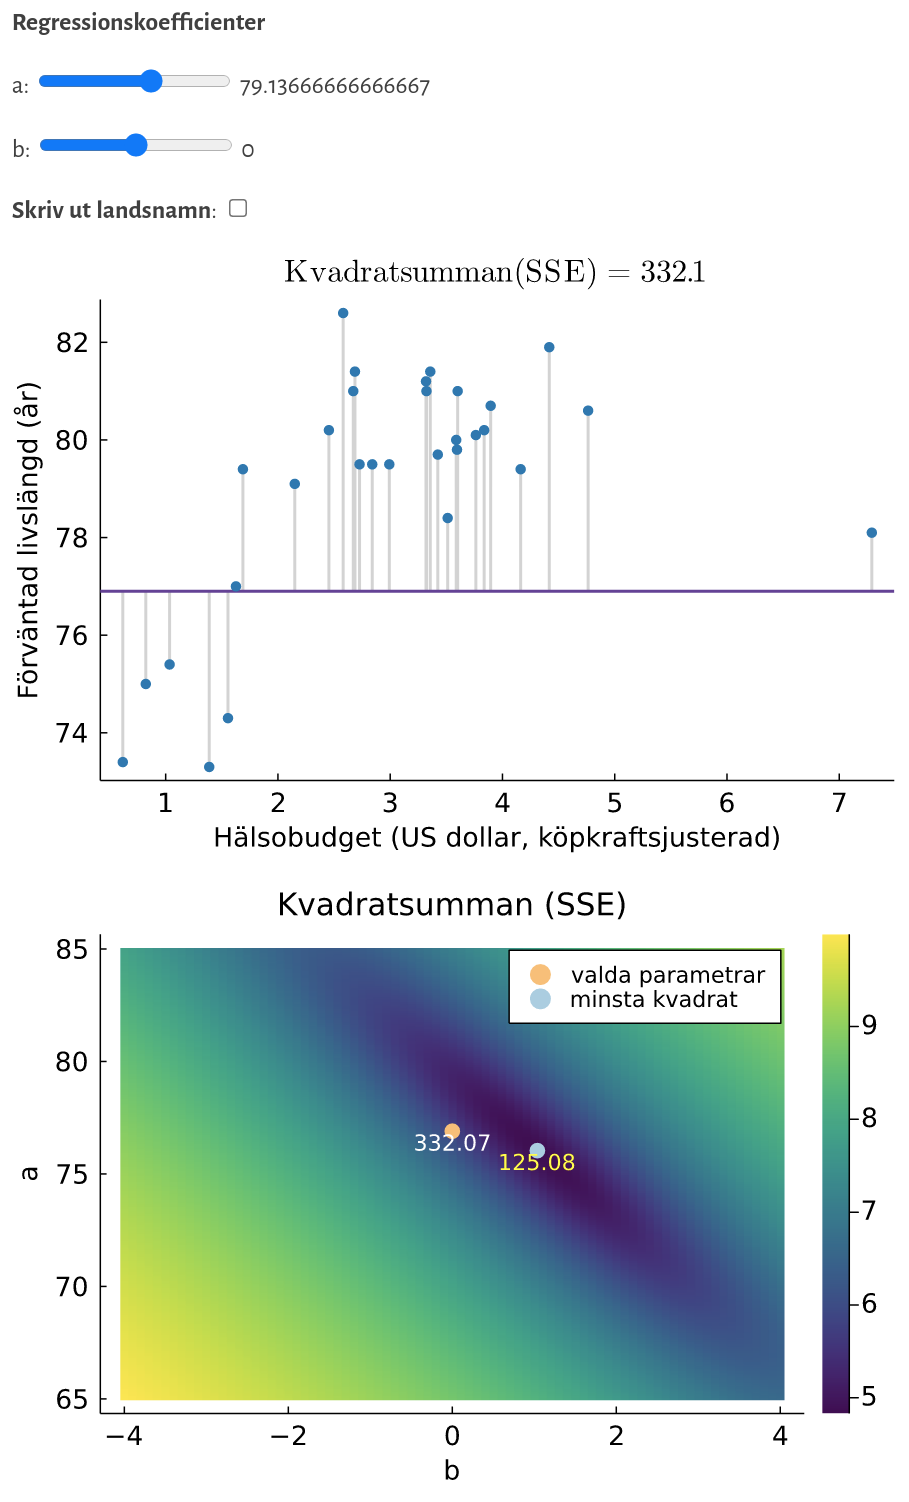
\includegraphics[viewport=0bp 620bp 909bp 1502bp,clip,scale=0.12]{figs/LeastSquaresPluto1}\qquad{}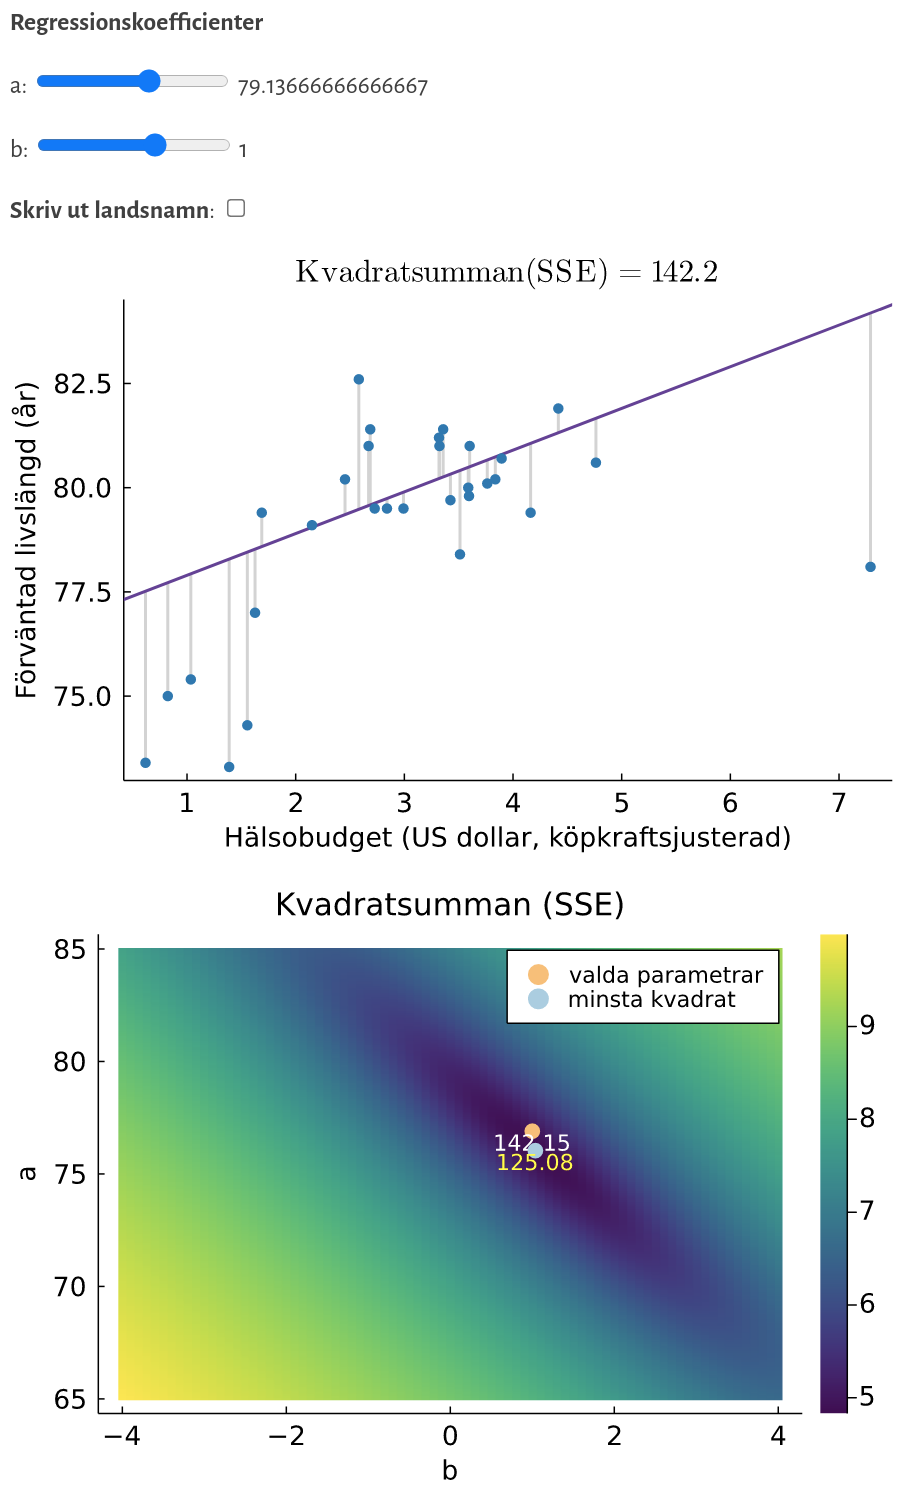
\includegraphics[viewport=0bp 620bp 905bp 1493bp,clip,scale=0.12]{figs/LeastSquaresPluto3}
%
\par\end{center}
\end{frame}

\begin{frame}{\textbf{\textcolor{orange}{Regression i R}}}
\begin{center}
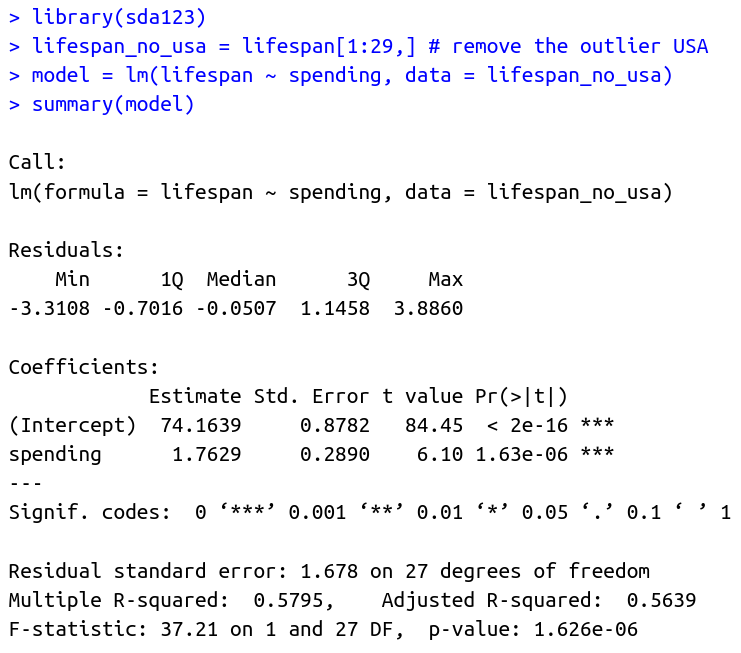
\includegraphics[scale=0.35]{figs/regression_in_R}
\par\end{center}

\end{frame}

\begin{frame}{\textbf{\textcolor{orange}{Residualvarians}}}
\begin{itemize}
\item \textbf{\textcolor{blue}{Residualvariansen }}- hur bra regressionslinjen
passar data:
\[
s_{e}^{2}=\frac{\sum_{i=1}^{n}(y_{i}-\hat{y}_{i})^{2}}{n-2}
\]
\item Kom ihåg: stickprovsvariansen delar med $n-1$ eftersom vi måste beräkna
$\bar{y}$ först:
\[
s_{y}^{2}=\frac{\sum_{i=1}^{n}(y_{i}-\bar{y})^{2}}{n-1}
\]
\item Residualvariansen delar med $n-2$ eftersom vi måste beräkna både
$b_{0}$ och $b_{1}$ först. \textbf{\textcolor{blue}{Väntevärdesriktig}}.
\bigskip{}
\item \textbf{\textcolor{blue}{Residualstandardavvikelsen}} (\texttt{\footnotesize{}residual
standard error}{\footnotesize{} i R})
\[
s_{e}=\sqrt{s_{e}^{2}}
\]
\item Hälsobudgetdata
\[
s_{e}^{2}=\frac{76.056}{29-2}\approx2.817\quad\quad\quad s_{e}=\sqrt{2.817}\approx1.678\mathrm{\text{ år}}
\]
\end{itemize}
\end{frame}

\begin{frame}{\textbf{\textcolor{orange}{Regression som sannolikhetsmodell}}}
\begin{itemize}
\item \textbf{\textcolor{blue}{Populationsmodell}} för enkel regression:
\[
Y=\beta_{0}+\beta_{1}x+\varepsilon,\quad\varepsilon\sim N(0,\sigma_{\varepsilon}^{2})
\]
\item $\beta_{0}$ är interceptet i populationen/modellen.\smallskip{}
\item $\beta_{1}$ är lutningen på regressionslinjen i populationen.\smallskip{}
\item \textbf{\textcolor{blue}{Regressionlinjen}} i populationen är ett
\textbf{\textcolor{blue}{betingat väntevärde}}:
\[
E(Y\vert x)=\beta_{0}+\beta_{1}x
\]
\item $\beta_{1}$ : hur $Y$ förändras \textbf{\textcolor{blue}{i genomsnitt}}
när $x$ ökar med en enhet.\smallskip{}
\item “i genomsnitt” = (betingat) väntevärde.\smallskip{}
\item Responsvariabeln $y$ kommer avvika från populationens regressionslinje
med en \textbf{\textcolor{blue}{slumpmässig “felterm” $\varepsilon$}}.\smallskip{}
\end{itemize}
\end{frame}

\begin{frame}{\textbf{\textcolor{orange}{Regression som modell för betingad fördelning}}}
\begin{center}
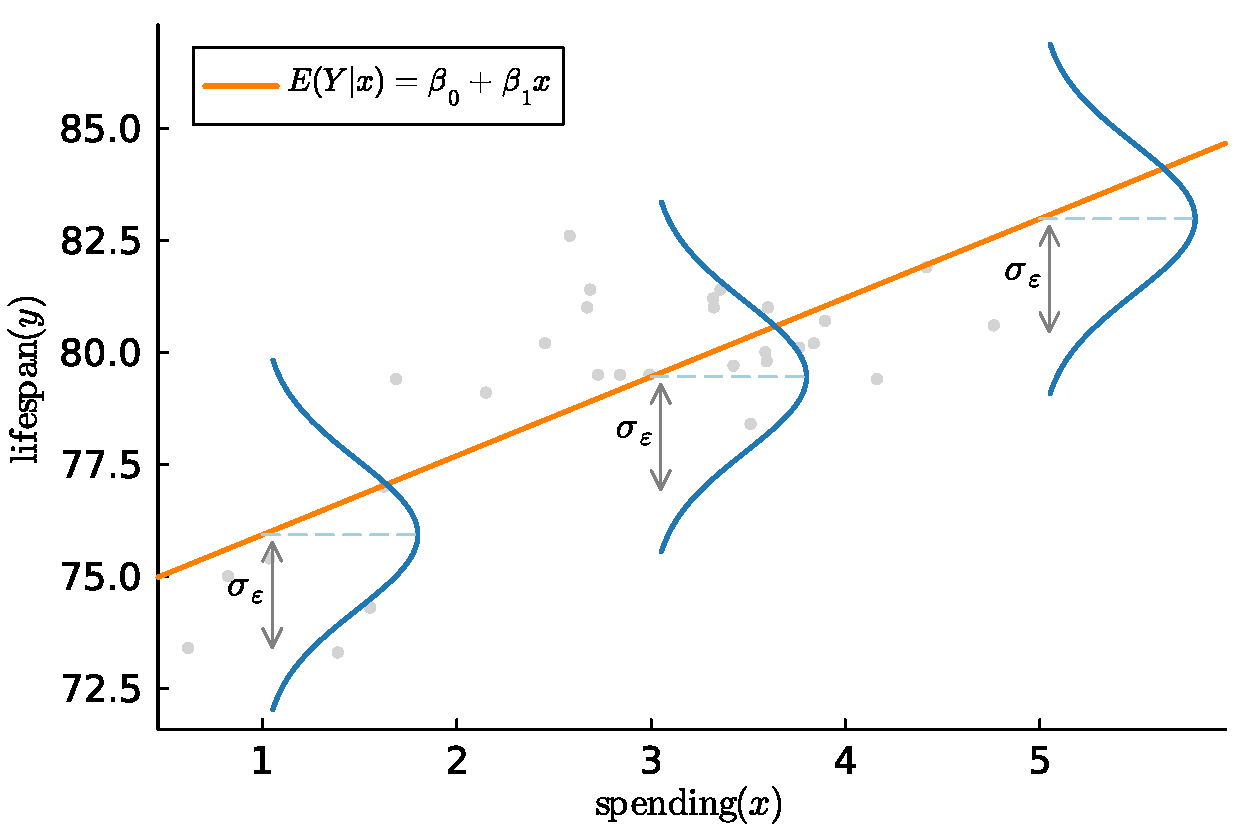
\includegraphics[scale=0.45]{figs/regdensities}
\par\end{center}

\end{frame}

\begin{frame}{\textbf{\textcolor{orange}{Regression som sannolikhetsmodell}}}
\begin{itemize}
\item \textbf{\textcolor{blue}{Populationsmodell}} för hela stickprovet:
\[
Y_{i}=\beta_{0}+\beta_{1}x_{i}+\varepsilon_{i},\quad\varepsilon_{i}\sim N(0,\sigma_{\varepsilon})
\]
\smallskip{}
\item \textbf{\textcolor{blue}{Stickprov/datamaterial}} med $n$ observationspar
\[
(y_{1},x_{1}),\ldots,(y_{n},x_{n})
\]
\smallskip{}
\item I regression antar vi att \textbf{\textcolor{blue}{$x$-variabeln
inte är slumpmässig}}. 
\end{itemize}
\end{frame}

\begin{frame}{\textbf{\textcolor{orange}{Residualerna $e_{i}$ skattar populationens
$\varepsilon_{i}$}}}
\begin{itemize}
\item \textbf{\textcolor{blue}{Residualer}}:
\[
e_{i}=y_{i}-\hat{y}_{i}
\]
\end{itemize}
\begin{center}
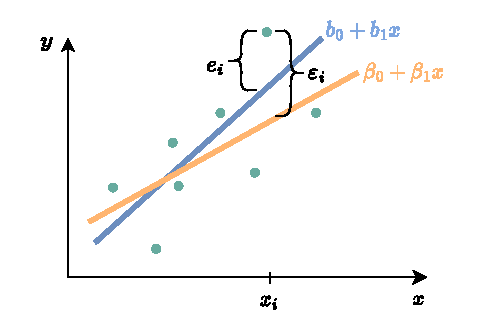
\includegraphics[scale=1.1]{figs/epsilon_vs_residual}
\par\end{center}
\begin{itemize}
\item Mer om detta på SDA2.
\end{itemize}
\end{frame}

\begin{frame}{\textbf{\textcolor{orange}{De fyra antaganden om populationen i regression}}}
\begin{enumerate}
\item Sambandet mellan $y$ och $x$ är \textbf{\textcolor{blue}{linjärt}}
\[
E(Y\vert x)=\beta_{0}+\beta_{1}x
\]
\item \textbf{\textcolor{blue}{Feltermerna}} \textbf{\textcolor{blue}{$\varepsilon_{i}$
är oberoende}} \bigskip{}
\bigskip{}
\item Feltermerna har \textbf{\textcolor{blue}{samma standardavvikelse}}
(homoskedastisk)
\[
SD(\varepsilon_{i})=\sigma_{\varepsilon}
\]
\item \textbf{\textcolor{blue}{Feltermerna är normalfördelade}}
\[
\varepsilon_{1},\ldots,\varepsilon_{n}\overset{\mathrm{ober}}{\sim}N(0,\sigma_{\varepsilon})
\]
\end{enumerate}
\end{frame}

\begin{frame}{\textbf{\textcolor{orange}{Residualanalys för att undersöka de 4 antagandena}}}
\begin{itemize}
\item \textbf{\textcolor{blue}{Residualer}}:
\[
e_{i}=y_{i}-\hat{y}_{i}
\]
\end{itemize}
\begin{enumerate}
\item \textbf{\textcolor{orange}{Linjärt samband?}} \\
\smallskip{}
Plotta $y_{i}$ mot $x_{i}$. Ser linjärt ut? \\
Plotta $e_{i}$ mot $x_{i}$. Konstant, eller mönster kvar?\bigskip{}
\item \textbf{\textcolor{orange}{Oberoende $\varepsilon$?}} \\
\smallskip{}
Plotta residualer $e_{i}$ mot anpassade värden $\hat{y}_{i}$. \\
Tidsserier: plotta $e_{i}$ mot tid (observationsnummer).\bigskip{}
\item \textbf{\textcolor{orange}{Homoskedastiska $\varepsilon$?}} \\
\smallskip{}
Plotta residualer $e_{i}$ mot $x_{i}$. Liknande spridning för alla
$x_{i}$?
\[
SD(\varepsilon_{i})=\sigma_{\varepsilon}
\]
\item \textbf{\textcolor{orange}{Normalfördelade $\varepsilon$?}} \\
\smallskip{}
Histogram, boxplot, QQ-plot för residualer $e_{i}$.
\end{enumerate}
\end{frame}

\begin{frame}{\textbf{\textcolor{orange}{Residualanalys lifespan - sda123-paketet\hspace{2cm}}}}
\begin{center}
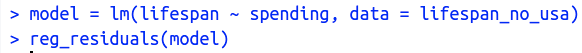
\includegraphics[scale=0.3]{figs/lifespan_reg_residual}
\par\end{center}

\begin{center}
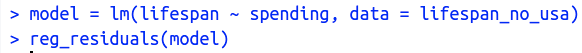
\includegraphics[scale=0.23]{figs/lifespan_reg_residual}
\par\end{center}

\end{frame}

\begin{frame}{\textbf{\textcolor{orange}{Residualer simulerade data - alla antaganden
OK}}}
\begin{center}
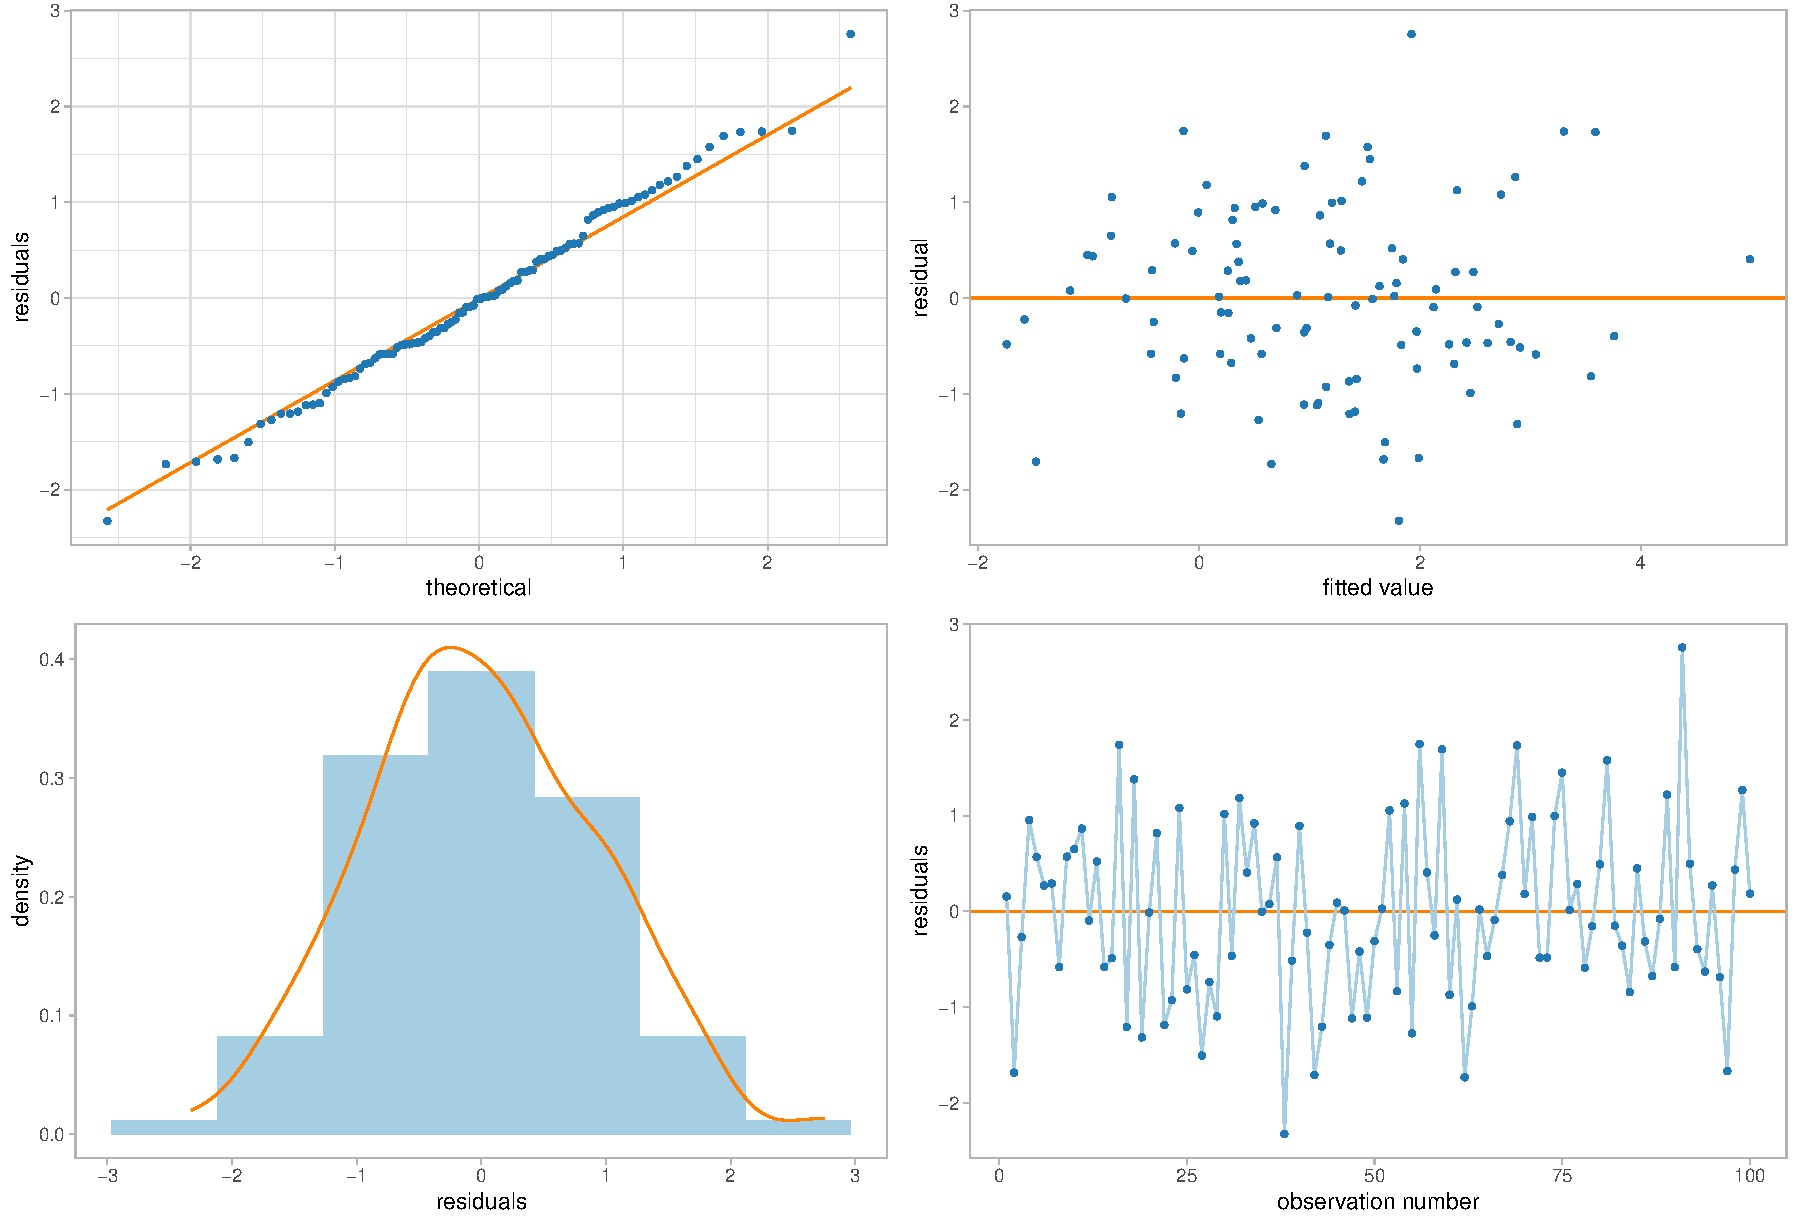
\includegraphics[scale=0.35]{figs/Residuals_AllGood}
\par\end{center}

\end{frame}

\begin{frame}{\textbf{\textcolor{orange}{Trouble in paradise 1 - heteroscedastisk
varians}}}
\begin{center}
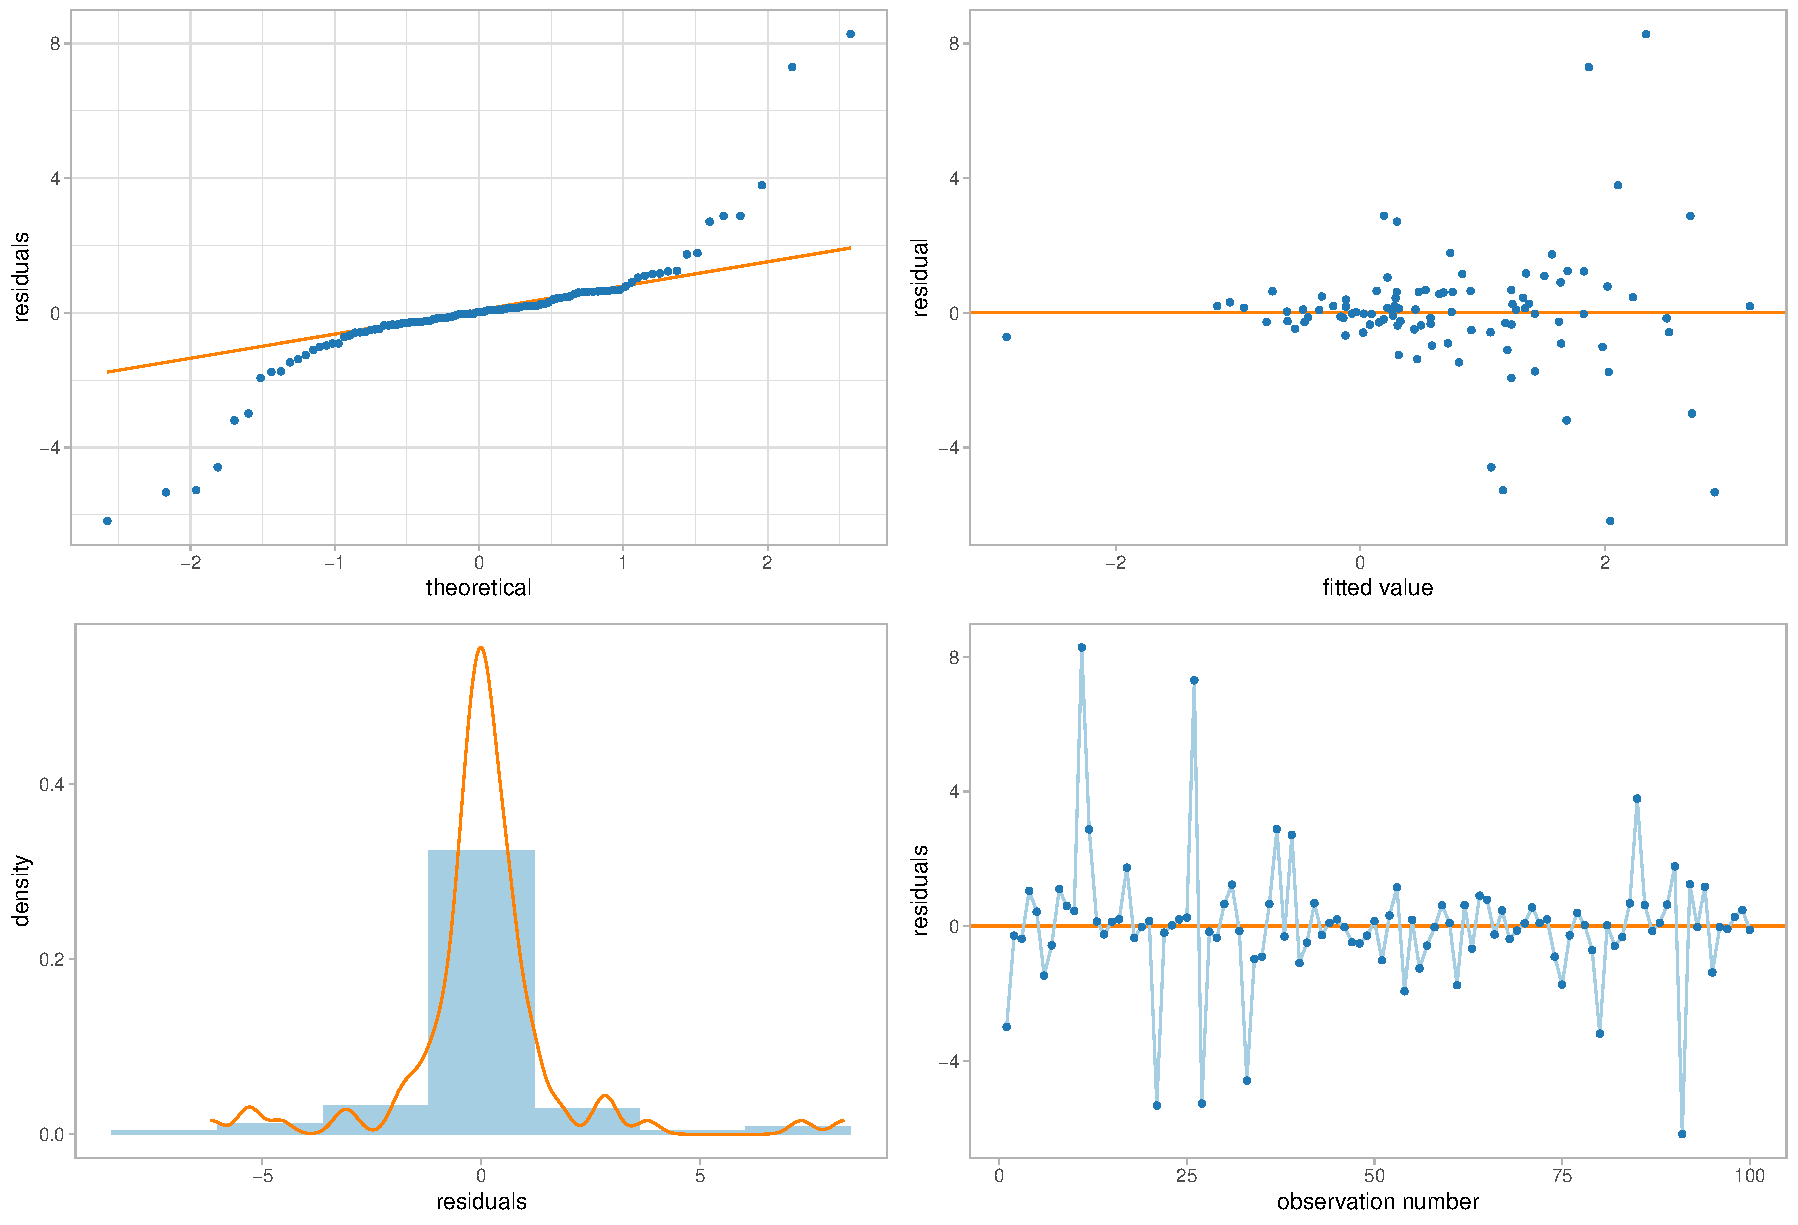
\includegraphics[scale=0.35]{figs/Residuals_NormalHetero}
\par\end{center}

\end{frame}

\begin{frame}{\textbf{\textcolor{orange}{Trouble in paradise 2 - icke-normala $\varepsilon$
(outliers)}}}
\begin{center}
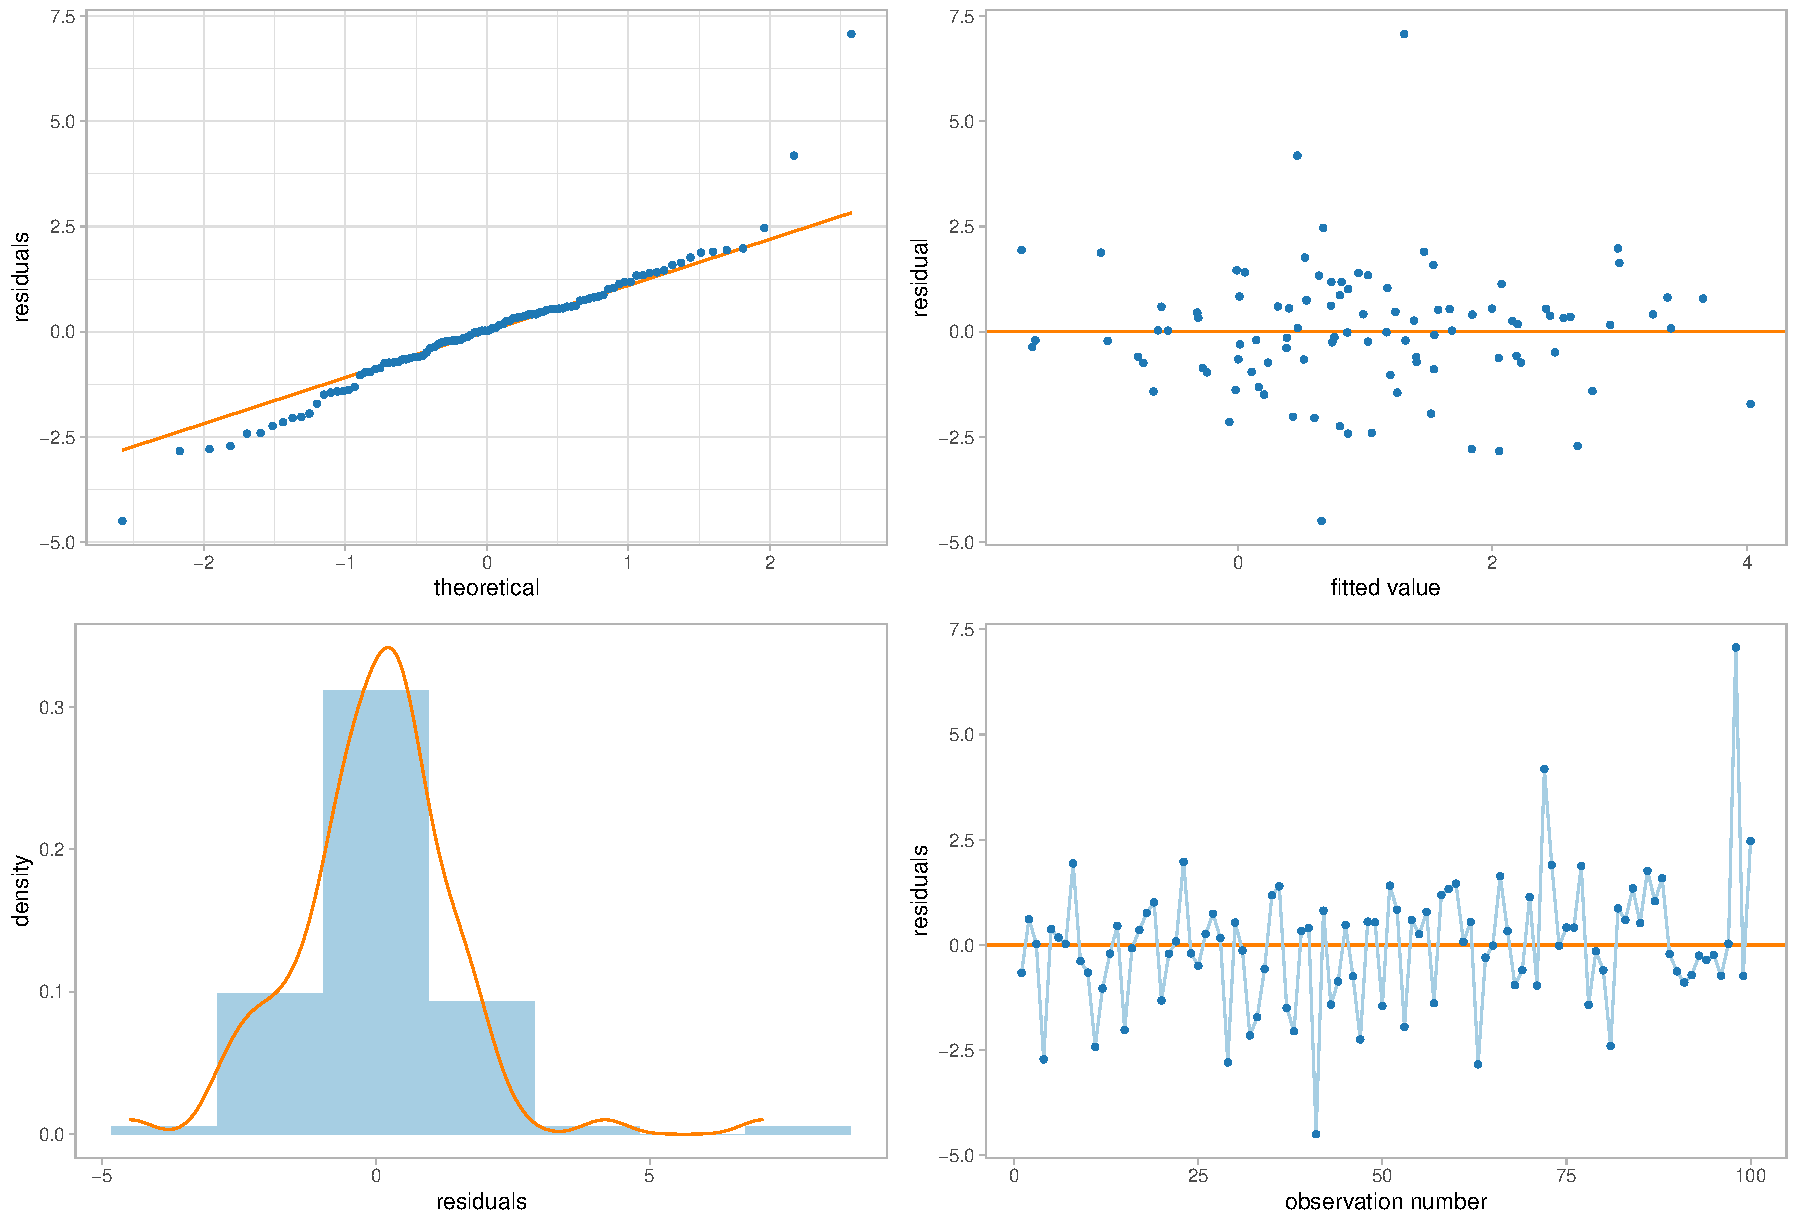
\includegraphics[scale=0.35]{figs/Residuals_Studentt4_Homo}
\par\end{center}

\end{frame}

\begin{frame}{\textbf{\textcolor{orange}{Trouble in paradise 3 - icke-normala och
hetero $\varepsilon$}}}
\begin{center}
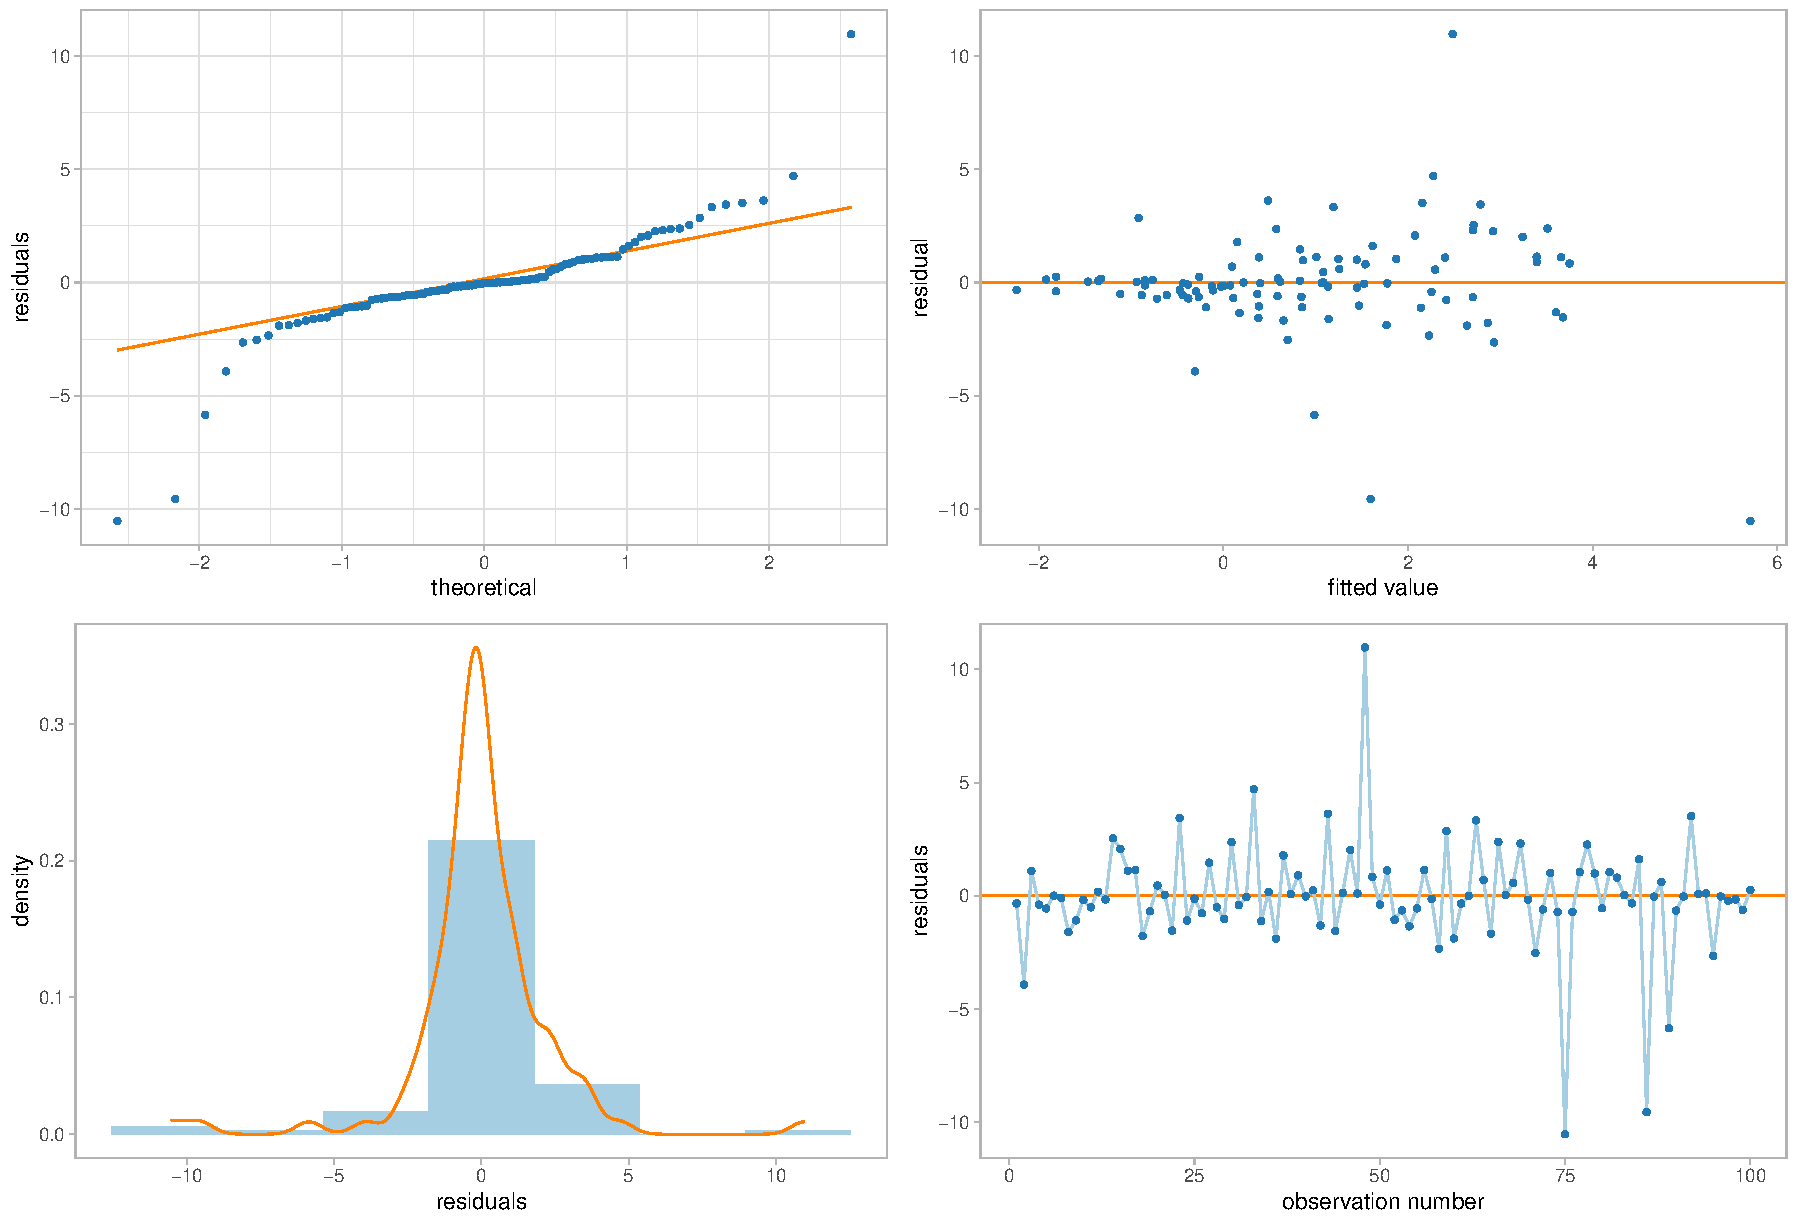
\includegraphics[scale=0.35]{figs/Residual_Studentt4_Hetero}
\par\end{center}

\end{frame}

\begin{frame}{\textbf{\textcolor{orange}{Trouble in paradise 4 - ej oberoende $\varepsilon$}}}
\begin{center}
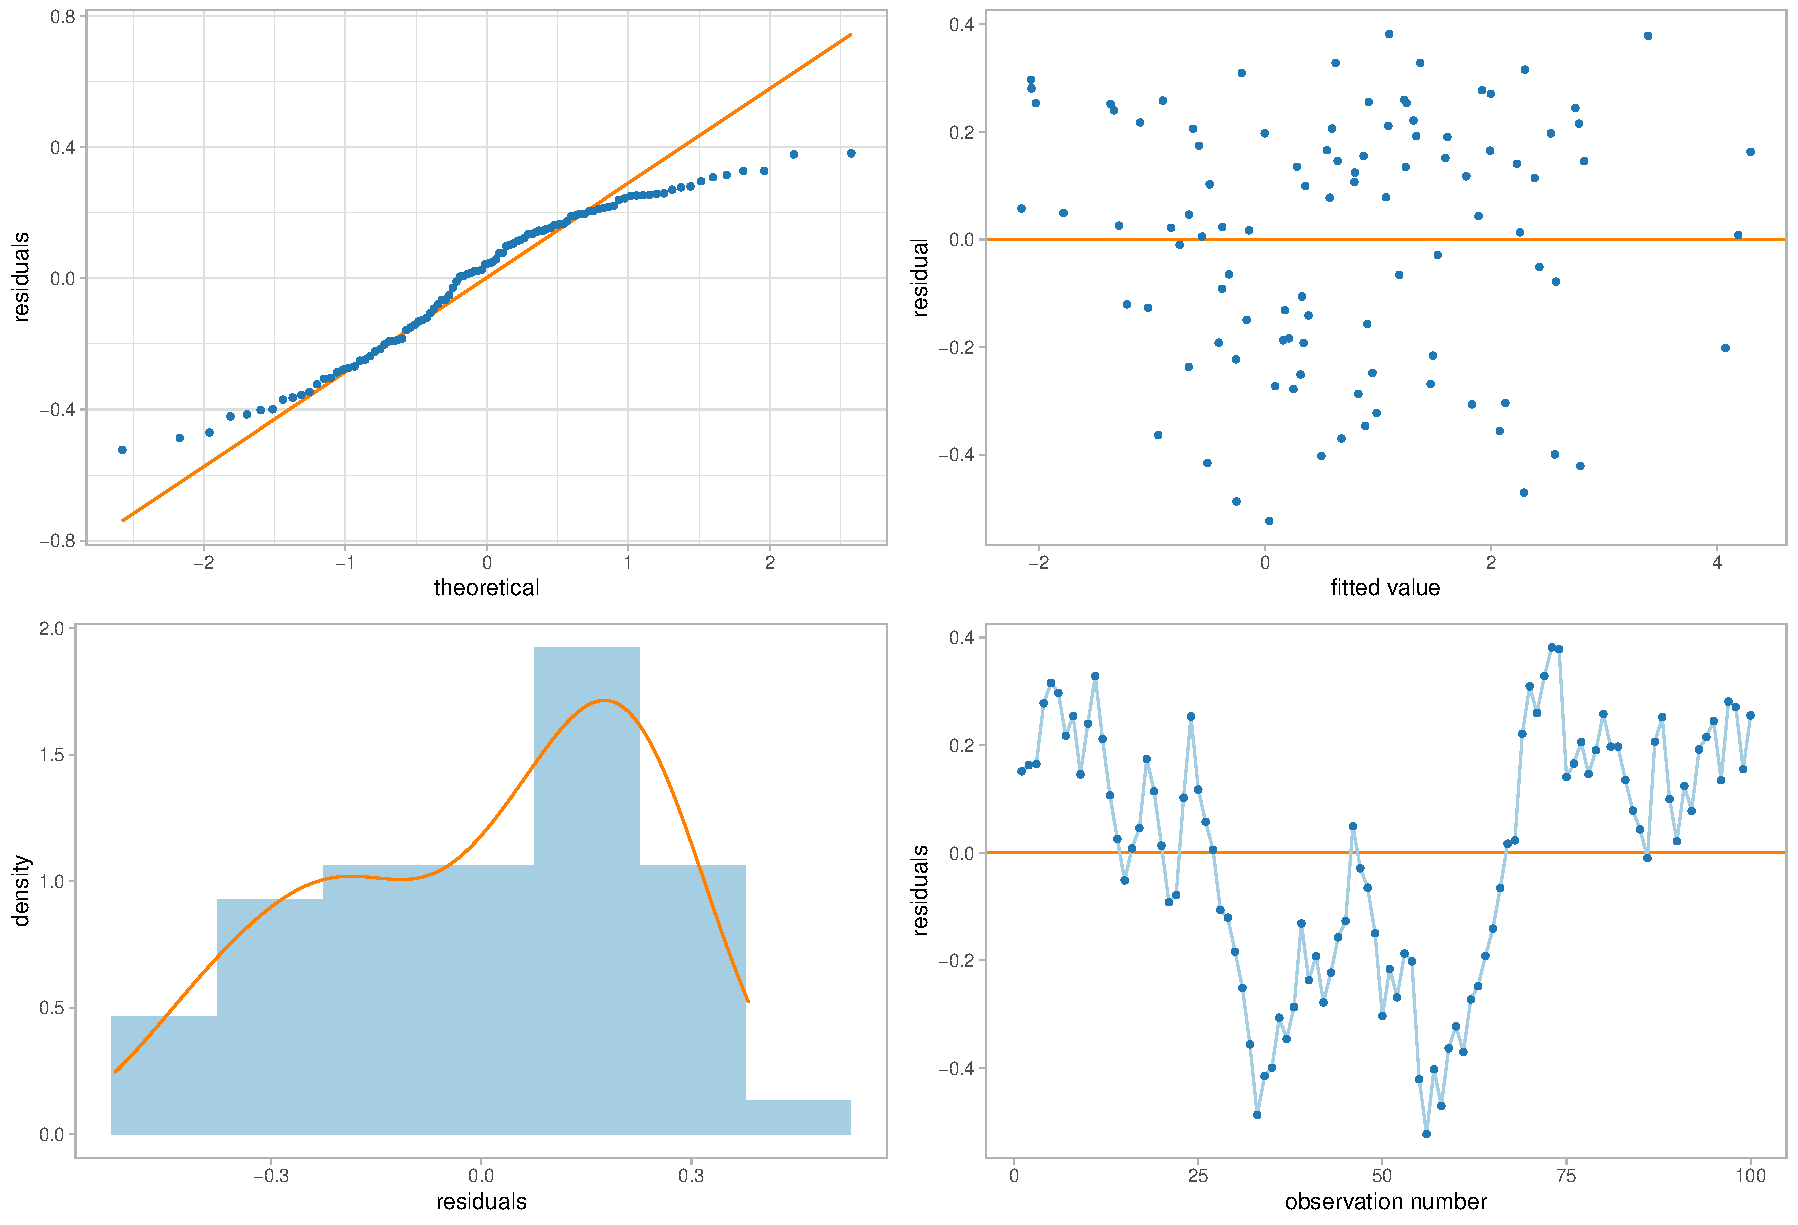
\includegraphics[scale=0.35]{figs/Residuals_Autocorrelated}
\par\end{center}

\end{frame}

\begin{frame}{\textbf{\textcolor{orange}{Minsta kvadrat-skattningar är väntevärdesriktiga}}}
\begin{itemize}
\item Minsta kvadrat-estimatorerna:
\[
b_{1}=\frac{s_{xy}}{s_{x}^{2}}
\]
\medskip{}
\[
b_{0}=\bar{y}-b_{1}\bar{x}
\]
\medskip{}
\end{itemize}
\[
s_{e}^{2}=\frac{\sum_{i=1}^{n}(y_{i}-\hat{y}_{i})^{2}}{n-2}
\]
\medskip{}

\begin{itemize}
\item \textbf{\textcolor{blue}{Väntevärdesriktiga}}\textcolor{black}{
\begin{align*}
E(b_{0}) & =\beta_{0}\\
E(b_{1}) & =\beta_{1}\\
E(s_{e}^{2}) & =\sigma_{\varepsilon}^{2}
\end{align*}
}
\end{itemize}
\end{frame}

\begin{frame}{\textbf{\textcolor{orange}{Standardfel för $b_{1}$}}}
\begin{itemize}
\item Estimatorn för lutningskoefficienten
\[
b_{1}=\frac{s_{xy}}{s_{x}^{2}}
\]
\item Hur $b_{1}$ varierar mellan olika stickprov:
\[
\sigma_{b_{1}}=SD(b_{1})=\frac{\sigma_{\varepsilon}}{\sqrt{n-1}s_{x}}
\]
\item $\sigma_{b_{1}}$ skattas med \textbf{\textcolor{blue}{standardfelet}}
\[
s_{b_{1}}=SE(b_{1})=\frac{s_{e}}{\sqrt{n-1}s_{x}}
\]
\item \textcolor{black}{Formel för $SE(b_{0})$ slipper ni på SDA1.\emoji{grinning-face-with-sweat}\smallskip{}
}
\item \texttt{lifespan} data \texttt{{[}sd(spending) = 1.09751}6{]}
\[
s_{b_{1}}=\frac{1.678}{\sqrt{29-1}\cdot1.097516}\approx0.289
\]
\end{itemize}
\end{frame}

\begin{frame}{\textbf{\textcolor{orange}{Standardfel för $b_{1}$ i R}}}
\begin{center}
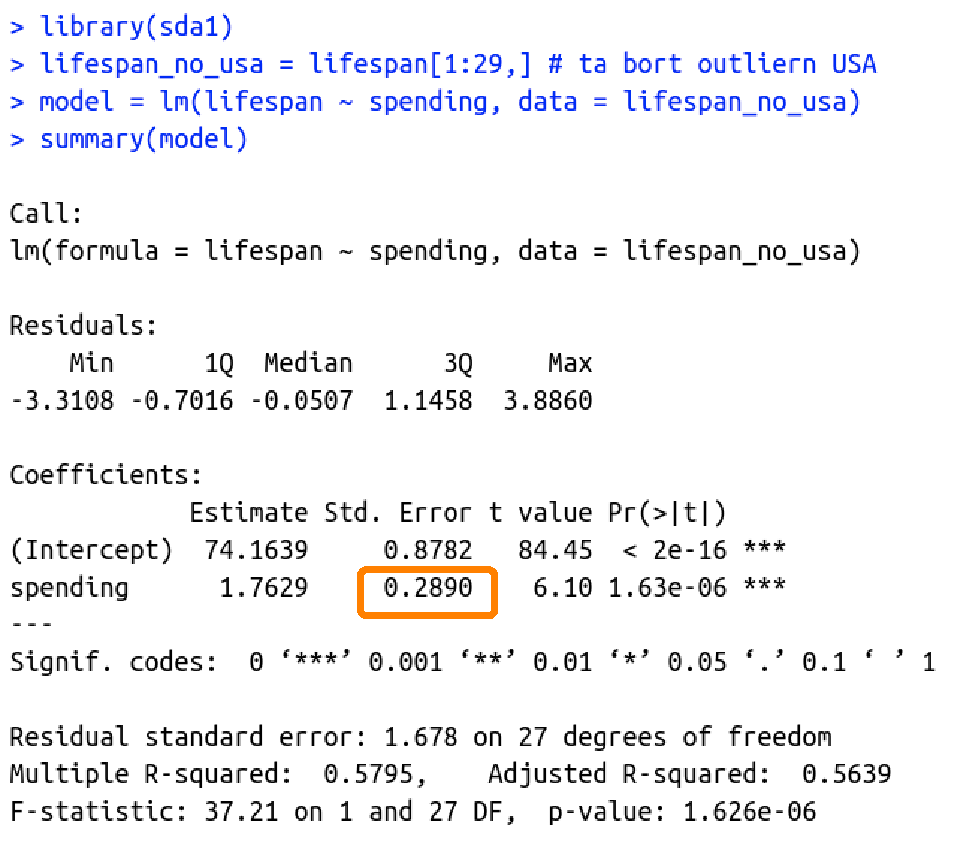
\includegraphics[scale=0.55]{figs/lifespan_reg_sterr}
\par\end{center}

\end{frame}

\begin{frame}{\textbf{\textcolor{orange}{Samplingfördelning i regression - interaktivt}}}
\begin{center}
\noindent{\fboxrule 1pt\fboxsep 1pt\fcolorbox{orange}{white}{\begin{minipage}[t]{1\columnwidth - 2\fboxsep - 2\fboxrule}%
\begin{center}
\href{https://statisticssu.github.io/SDA1/observable/linreg_simple_sampling_dist.html}{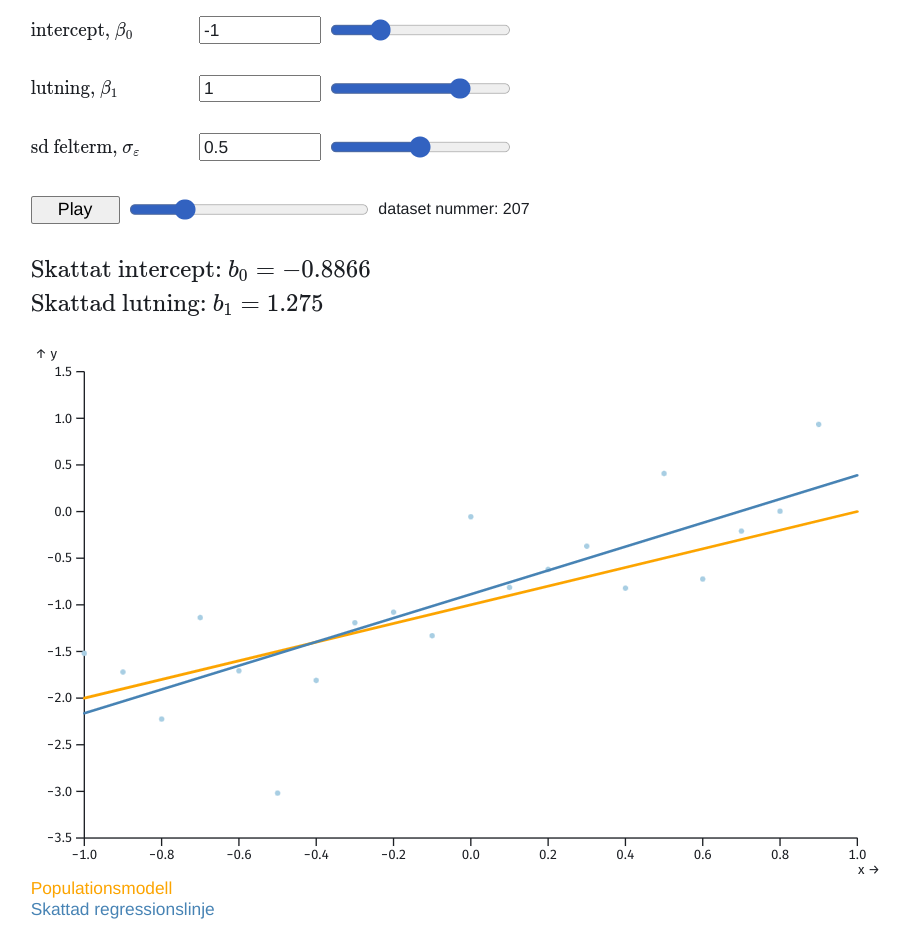
\includegraphics[width=0.6\textwidth]{figs/sampdist_regression_widget.png}}
\par\end{center}%
\end{minipage}}}
\par\end{center}

\end{frame}

\begin{frame}{\textbf{\textcolor{orange}{Credits}}}
\end{frame}

\subsubsection*{Dessa slides skapades för kursen statistik och dataanalys 1 av Mattias
Villani HT 2023, och har modifierats av Oscar Oelrich VT 2024, och
Oskar Gustafsson för VT 2025.}
\end{document}
